% Slide 2: Project Context & Problem Statement
\begin{frame}{Project Context}
    \begin{itemize}
        \item \textbf{Objective:} Simulate a dynamic environment where periodic tasks are activated/deactivated via a remote supervisor (Client) through a central controller (Server).
        \item \textbf{System Model:}
        \begin{itemize}
            \item \textbf{Server:} Manages a pool of clients and a pool of real-time worker threads.
            \item \textbf{Clients:} Issue commands to modify the system state (Activate, Deactivate,     Block, Stop, Quit).
            \item \textbf{Tasks:} Periodic routines with predefined execution times, deadlines and periods.
        \end{itemize}
        \item \textbf{The Challenge:} Managing high-frequency state changes across multiple threads (Connection Handlers, Task Workers, and the Main Server Loop) without incurring race conditions or deadlocks.
    \end{itemize}
\end{frame}

% Slide 3: Architectural Overview
\begin{frame}{System Architecture}
    \centering
    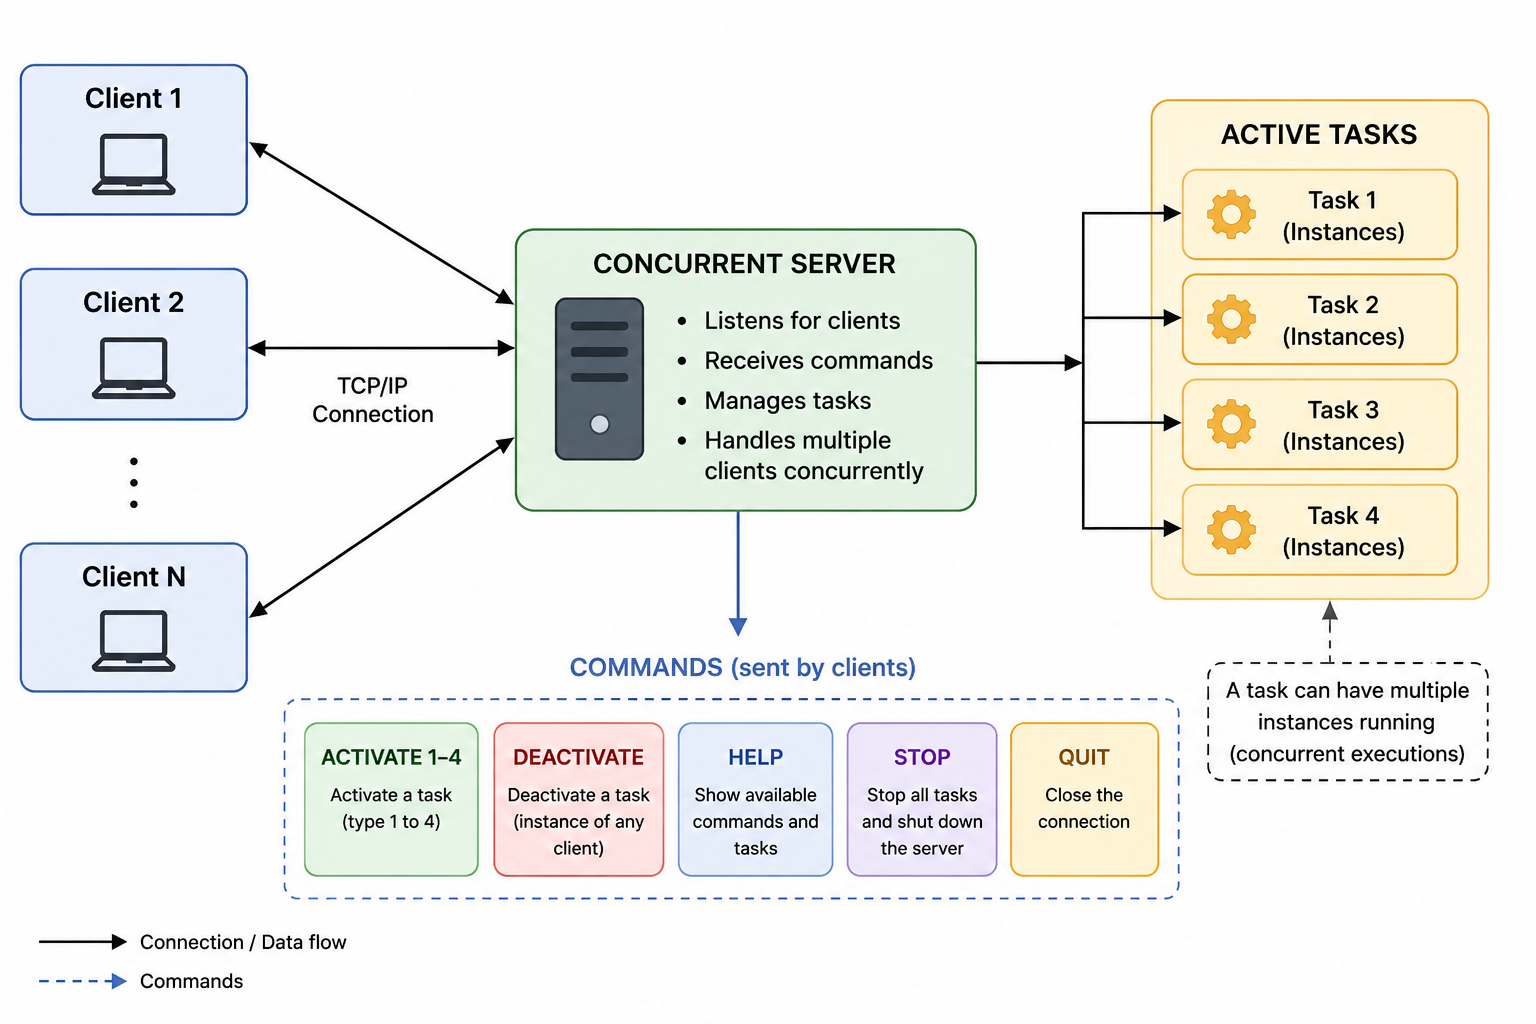
\includegraphics[width=0.75\textwidth]{images/image.png}
    
    \vspace{0.3cm}
    \begin{itemize}
        \item \textbf{Decoupled Design:} Separates network connection handling from real-time task execution.
        \item \textbf{1:1 Thread Mapping:} One \textit{Connection Handler} per client socket; one \textit{Worker Thread} per active task instance.
    \end{itemize}
\end{frame}



% Slide 4: Data Structure Analysis
\begin{frame}{Core Data Structures}
    To ensure thread safety, the system relies on two primary shared arrays:
    \begin{enumerate}
        \item \texttt{Client clients[MAX\_THREADS]}:
        \begin{itemize}
            \item Tracks connected clients, their socket FDs, and assigned ports.
            \item \textbf{Protected by:} \texttt{mutex\_clients\_array}, \texttt{roomAvailable}.
        \end{itemize}
        \item \texttt{ActiveTask tasks\_active[MAX\_NUMBER\_ACTIVE\_TASKS]}:
        \begin{itemize}
            \item Tracks currently running periodic tasks, their IDs, and thread handles.
            \item \textbf{Protected by:} \texttt{active\_tasks\_mutex}, \texttt{free\_slots\_sem}.
        \end{itemize}
    \end{enumerate}
    \vspace{0.3cm}
    \textit{Note: These structures represent the "Critical Sections" where race conditions are most likely to occur during simultaneous command processing.}
\end{frame}

% Synchronization Strategy: Mutexes
\begin{frame}{Mutexes}
    The implementation utilizes several \texttt{pthread\_mutex\_t} objects to enforce Mutual Exclusion:
    \begin{description}
        \item[\texttt{mutex\_clients\_array}] Protects the integrity of the client registry. Ensures only one thread modifies the client list at a time.
        \item[\texttt{active\_tasks\_mutex}] Protects the task registry. Critical for preventing corruption when tasks are added or removed.
        \item[\texttt{mutex\_stopserver}] Protects the global shutdown flag, preventing a race between the "Stop" command and the main loop's exit condition.
        \item[\texttt{log\_mutex}] \textbf{Output Integrity:} Essential for real-time debugging. Prevents multiple threads from interleaving their \texttt{printf} calls, which would render the server logs unreadable.
    \end{description}
\end{frame}

% Synchronization Strategy: Condition Variables
\begin{frame}{Condition Variables}

    To handle the ``Server Full'' state for clients, we employ
    \texttt{pthread\_cond\_t} (\texttt{roomAvailable}):

    \begin{itemize}

        % \item \textbf{The Producer (Server Loop):}
        % When a new connection arrives via \texttt{accept()}, the server
        % attempts to add the client.

        \item \textbf{The Consumer (Connection Handler):}
        If \texttt{findFreePosition()} returns $-1$ (Server's array for client is full), the
        thread enters:

        \begin{itemize}
            \item \texttt{pthread\_mutex\_lock(\&mutex\_clients\_array)}
            \item \texttt{pthread\_cond\_wait(\&roomAvailable,
            \&mutex\_clients\_array)}
        \end{itemize}

        \item \textbf{The Signal:}
        When \texttt{rmvclient()} is called (a client disconnects),
        \texttt{pthread\_cond\_signal(\&roomAvailable)} is invoked,
        waking up a waiting thread so it can occupy the newly available
        slot.

    \end{itemize}

\end{frame}


% Synchronizatio Strategy: Semaphores
\begin{frame}{Semaphores}
    The system uses a \textbf{Counting Semaphore} (\texttt{free\_slots\_sem}) to manage the \texttt{tasks\_active} array:
    \begin{itemize}
        \item \textbf{Initialization:} \texttt{sem\_init(\&free\_slots\_sem, 0, MAX\_NUMBER\_ACTIVE\_TASKS)}.
        \item \textbf{Resource Tracking:} The semaphore acts as a counter for available slots.
        \item \textbf{Non-Blocking Allocation:} 
        \begin{itemize}
            \item \texttt{sem\_trywait} is used during activation. 
            \item If the semaphore is 0 (no slots), the server immediately rejects the task with a \texttt{FULL CAPACITY} message instead of hanging.
        \end{itemize}
        \item \textbf{Reclamation:} When a task is de-activated, \texttt{sem\_post} increments the counter, allowing the next \texttt{ACTIVATE} command to proceed.
    \end{itemize}
\end{frame}


% Slide 5: Command Logic: Activation
\begin{frame}{Command Logic: \texttt{ACTIVATE} Task}
    When a client sends an \texttt{ACTIVATE <ID>} command, the Server follows this protocol:
    \begin{enumerate}
        \item \textbf{Parsing:} Extract task ID from the command string.
        \item \textbf{Resource Acquisition:} 
        \begin{itemize}
            \item Attempt to decrement the \texttt{free\_slots\_sem}.
            \item Lock \texttt{active\_tasks\_mutex}.
            \item Locate an empty slot in \texttt{tasks\_active}.
        \end{itemize}
        \item \textbf{Schedulability Check:} Run \texttt{is\_schedulable()}. This is a read-only operation on the task array.
        \item \textbf{Thread Spawning:} Call \texttt{pthread\_create} for \texttt{handling\_active\_task}.
        \item \textbf{Unlock:} Release \texttt{active\_tasks\_mutex}.
    \end{enumerate}
\end{frame}

% Slide 6: Command Logic: Deactivation & Termination
\begin{frame}{Command Logic: \texttt{BLOCK}, \texttt{QUIT}, and \texttt{STOP}}
    \begin{itemize}
        \item \textbf{\texttt{BLOCK} (Deactivate Task):}
        \begin{itemize}
            \item Finds the oldest task instance in \texttt{tasks\_active}.
            \item Sets field of that task \texttt{active = 0} inside a \texttt{active\_tasks\_mutex} block.
            \item \textbf{Crucial:} The worker thread, seeing \texttt{active == 0}, terminates its loop.
            \item Calls \texttt{sem\_post} to signal a slot is now free.
        \end{itemize}
        \item \textbf{\texttt{QUIT} (Client Disconnect):}
        \begin{itemize}
            \item Closes the socket and calls \texttt{rmvclient()} which...
            \item Uses \texttt{mutex\_clients\_array} to update the client buffer.
        \end{itemize}
        \item \textbf{\texttt{STOP} (Global Shutdown):}
        \begin{itemize}
            \item Updates the global \texttt{close\_server} flag.
            \item \textbf{Synchronization:} Uses \texttt{mutex\_stopserver} to ensure atomic visibility of the shutdown signal to all threads.
        \end{itemize}
    \end{itemize}
\end{frame}





% Slide 11: Summary of Synchronization Primitives
\begin{frame}{Summary of Synchronization Primitives}
    \begin{table}
        \centering
        \small
        \begin{tabular}{|l|l|l|}
        \hline
        \textbf{Primitive} & \textbf{Variable Name} & \textbf{Synchronization Scope} \\ \hline
        Mutex & \texttt{mutex\_clients\_array} & Protects Client array state and slots \\ \hline
        Mutex & \texttt{active\_tasks\_mutex} & Protects Task array state insertion/deletion \\ \hline
        Mutex & \texttt{log\_mutex} & Ensures atomic, un-interleaved console logging \\ \hline
        Mutex & \texttt{mutex\_stopserver} & Prevents race conditions on shutdown flag \\ \hline
        Semaphore & \texttt{free\_slots\_sem} & Non-blocking task capacity tracking (\texttt{sem\_trywait}) \\ \hline
        Cond Var & \texttt{roomAvailable} & Blocks overflow clients until a slot frees up \\ \hline
        \end{tabular}
        \caption{Mapping of POSIX primitives to system critical sections.}
    \end{table}
\end{frame}

% Slide 12: Conclusion
\begin{frame}{Conclusion}
    \begin{itemize}
        \item \textbf{Robustness:} The system successfully bridges the gap between high-level TCP commands and low-level real-time thread management.
        \item \textbf{Concurrency Safety:} By utilizing mutexes for state, semaphores for resources and Condition Variables for flow control.
        \item \textbf{Scalability:} The architecture allows for $N$ clients and $M$ tasks to operate simultaneously, governed strictly by the defined synchronization boundaries.
    \end{itemize}
\end{frame}

\begin{frame}{Future Improvements}
    \begin{itemize}
        \item Compare Rate Monotonic with alternative fixed-priority policies.
        \item Extend evaluation to dynamic-priority algorithms (e.g., EDF).
        \item Evaluate system performance under high CPU utilization and overloaded conditions.
        \item Thread pool for clients achitecture.
        \item Possibly constant scan of all the clients and active tasks
    \end{itemize}
\end{frame}